\chapter{Antecedentes}\label{Appendix:Antecedentes}

El objetivo de este apéndice es que el lector conozca el crecimiento de las investigaciones
llevadas a cabo en el área de estudio de la presente tesis. Esto ayudará a comprender
y respaldar las motivaciones del presente trabajo.
Así, se podrá demostrar que existe una gran cantidad de investigadores
(los cuales se incrementan con el paso de los años), que se enfocan en la problemática a las cuales
se enfrenta esta tesis. Para ello, se utilizó la base de datos Scopus\footnote{www.scopus.com}, la cual es una
base de datos que contiene abstracts, citaciones, y artículos científicos. 

En primer lugar se realizó la búsqueda de las palabras claves ``COTS satellites'', obteniendo los resultados
que se muestran en la Figura \ref{fig:ant1}. Se observa que existe una tendencia creciente en las investigaciones
que contienen estas \textit{key words}.
Se encontró una cantidad total de 2047 artículos científicos. 

\begin{figure}[h!]
 \centering
 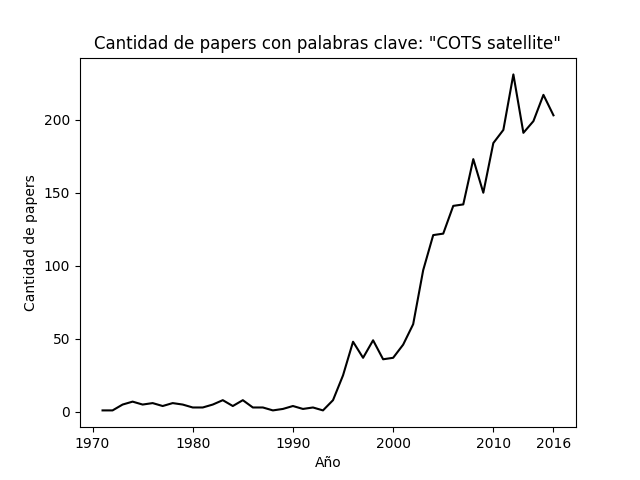
\includegraphics[scale=0.8]{images/Secciones/antecedentes/Cantidad_paper-COTS-Satellite.png}
  \caption{Cantidad de investigaciones con palabra clave ``COTS satellite''}
\label{fig:ant1}
\end{figure}

Por otro lado, se llevó a cabo una búsqueda de las mismas palabras claves, pero esta vez,
la consulta se realizó para conocer los principales países involucrados en estas investigaciones.
De esto, se obtiene el gráfico de la Figura \ref{fig:ant2}. Como se observa el país con más
investigaciones es Etados Unidos.

\begin{figure}[h!]
 \centering
 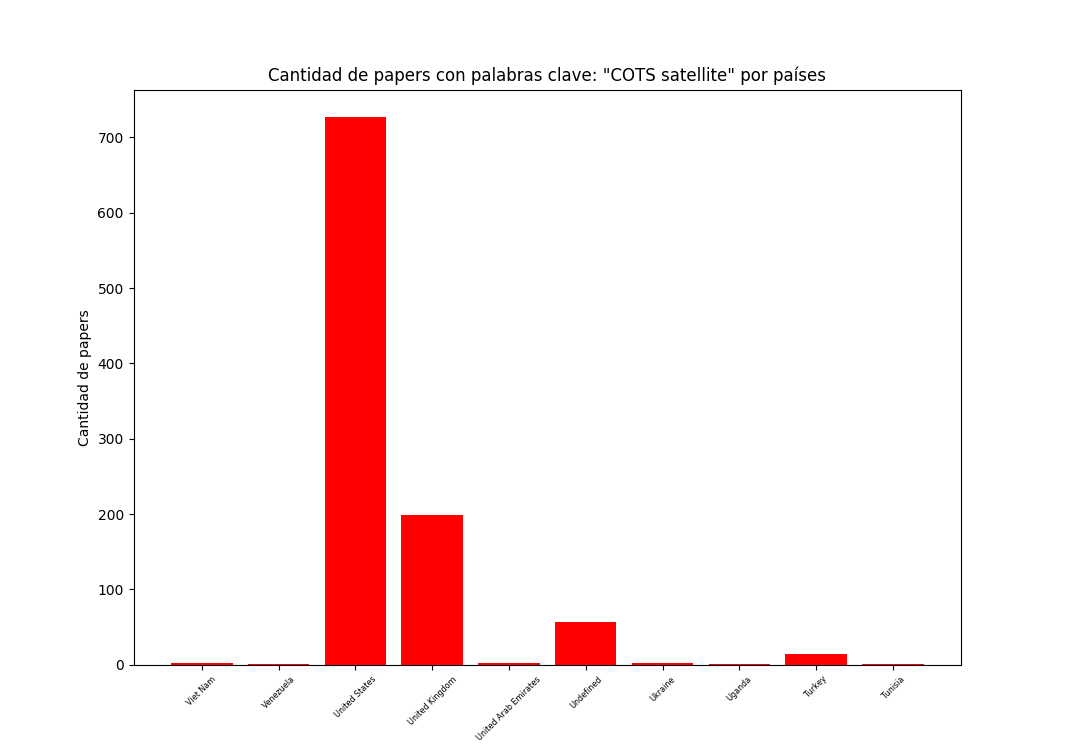
\includegraphics[scale=0.6]{images/Secciones/antecedentes/Cantidad_paper-COTS-Satellite-Country.png}
  \caption{Cantidad de investigaciones con palabra clave ``COTS satellite'' por países}
\label{fig:ant2}
\end{figure}

De la misma manera se realizó una consulta de las palabras claves: ``Fault Tolerance Satellite'',
para conocer tanto la cantidad de artículos existentes (Figura \ref{fig:ant3}). Nuevamente, se puede
observar un creciente interés en llevar a cabo investigaciones con respecto a las áreas de interés
de este trabajo de tesis. 

\begin{figure}[h!]
 \centering
 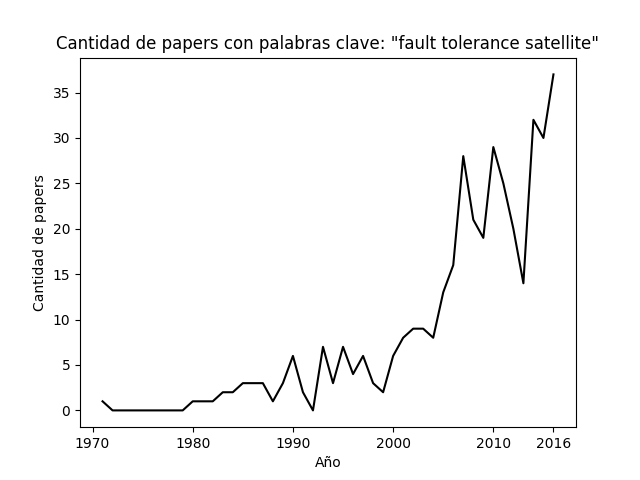
\includegraphics[scale=0.8]{images/Secciones/antecedentes/Cantidad_paper-fault_tolerance_satellite.png}
  \caption{Cantidad de investigaciones con palabra clave ``Fault Tolerance Satellite''}
\label{fig:ant3}
\end{figure}


Luego se realizó una búsqueda con las siguientes \textit{key words}: ``COTS Fault Tolerance''. Como resultado se obtuvo que existe una lateralización en la tendencia de las investigaciones en estas
áreas como se puede observar en la Figura \ref{fig:ant4}. Nuevamente, el país con más investigaciones
en el área sigue siendo Estados Unidos \ref{fig:ant5}. 


\begin{figure}[h!]
 \centering
 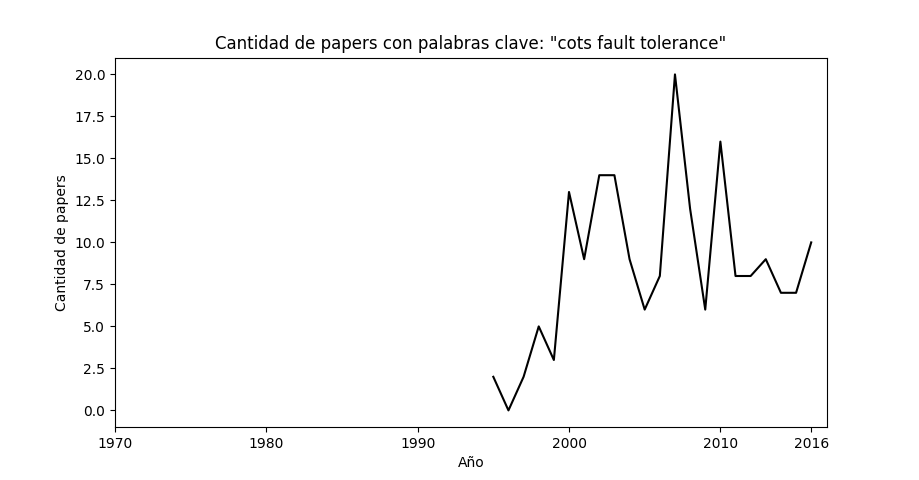
\includegraphics[scale=0.6]{images/Secciones/antecedentes/Cantidad_paper-COTS_fault_tolerance.png}
  \caption{Cantidad de investigaciones con palabra clave ``COTS Fault Tolerance'' }
\label{fig:ant4}
\end{figure}


\begin{figure}[h!]
 \centering
 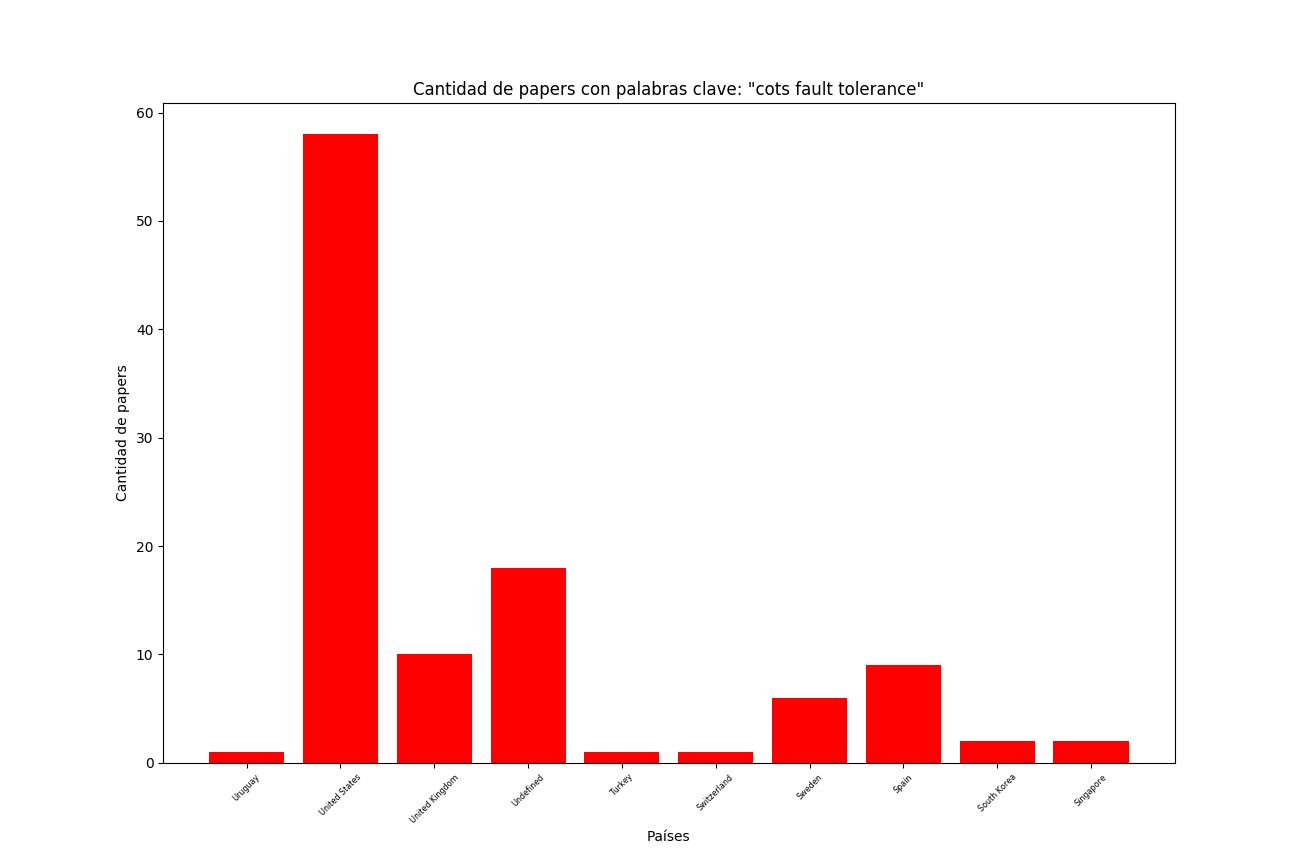
\includegraphics[scale=0.5]{images/Secciones/antecedentes/Cantidad_paper-COTS_fault_tolerance-Country.png}
  \caption{Cantidad de investigaciones con palabra clave ``COTS Fault Tolerance'' por países}
\label{fig:ant5}
\end{figure}

Por último se llevó a cabo una consulta con las palabras claves: ``Fault Tolerance Satellite
Architecture''. Los resultados se pueden observar en las Figuras \ref{fig:ant6} y \ref{fig:ant7}.
Como en las consultas anteriores, se observa un creciente interés por el estudio de esta área de
trabajo y el país como mayor publicación, sigue siendo Estados Unidos.



\begin{figure}[h!]
 \centering
 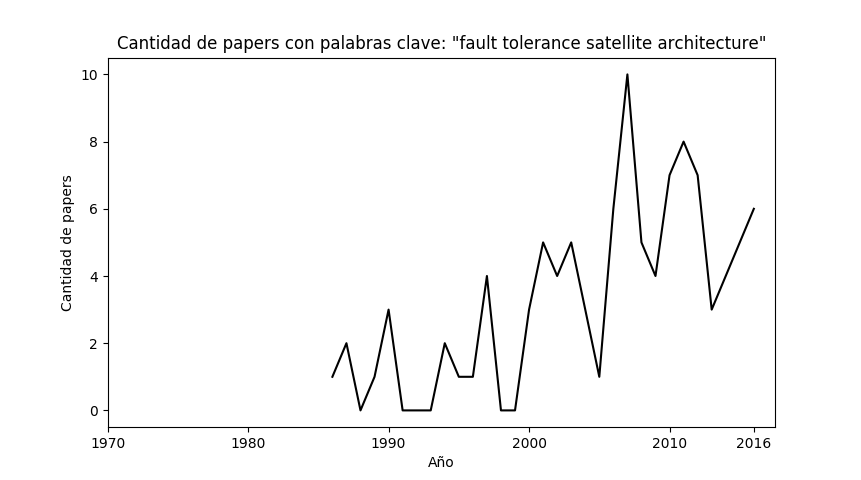
\includegraphics[scale=0.8]{images/Secciones/antecedentes/Cantidad_paper-fault_tolerance_satellite_architecture.png}
  \caption{Cantidad de investigaciones con palabra clave ``Fault Tolerance Satellite Architecture'' }
\label{fig:ant6}
\end{figure}


\begin{figure}[h!]
 \centering
 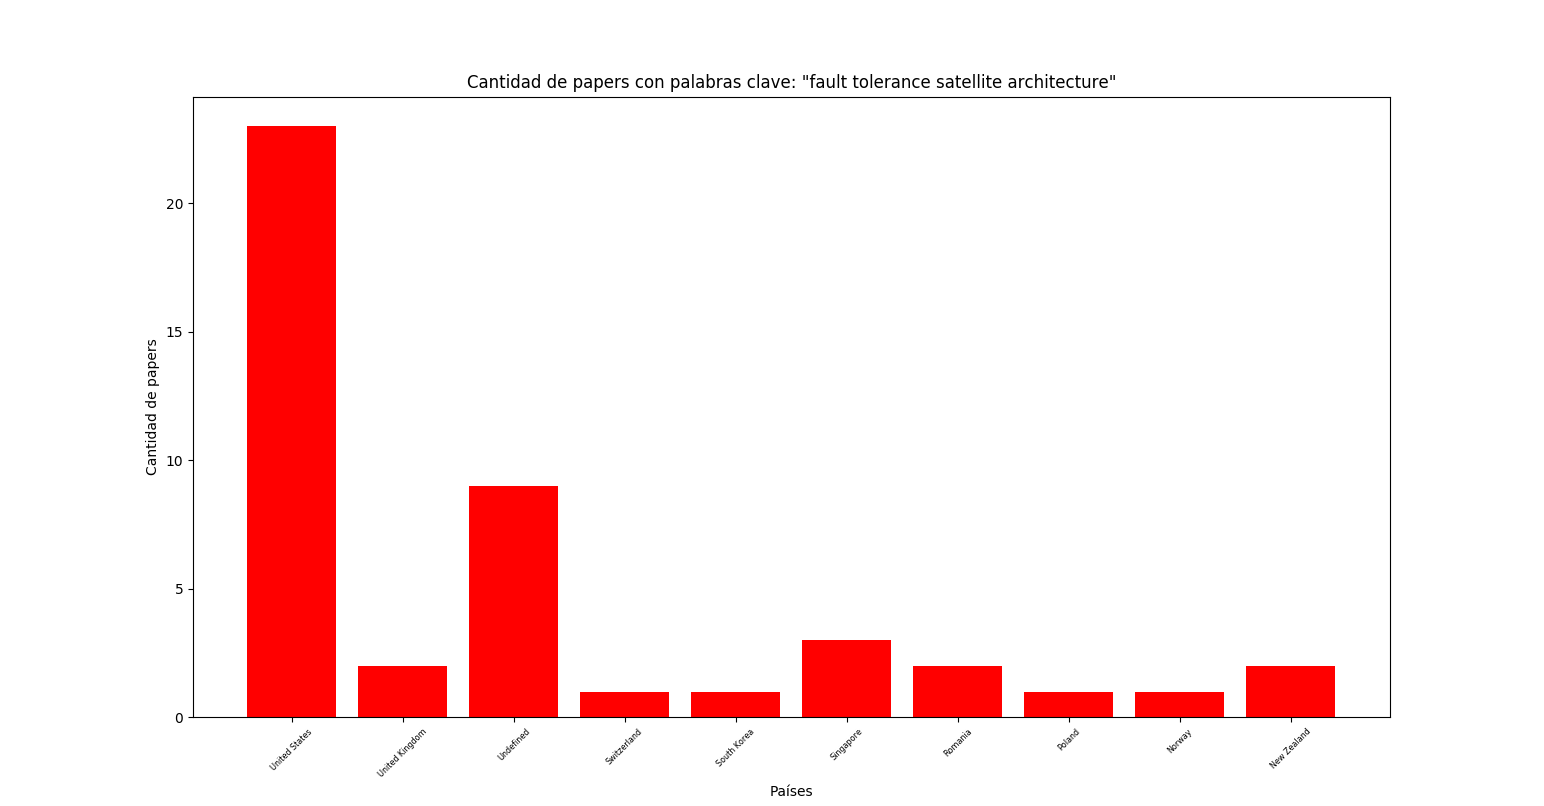
\includegraphics[scale=0.4]{images/Secciones/antecedentes/Cantidad_paper-fault_tolerance_satellite_architecture-Country.png}
  \caption{Cantidad de investigaciones con palabra clave ``Fault Tolerance Satellite Architecture'' por países}
\label{fig:ant7}
\end{figure}

De estas búsquedas sencillas, se puede llegar a la conclusión de que en general, existe una tendencia
creciente en investigaciones en el área que compete este trabajo de tesis. Además, se puede
obtener como conclusión de que existe una mayor cantidad de investigaciones en la dirección de
``COTS'' y ``Satellites''. Esto se puede justificar con la existencia de una necesidad de
reducir costos a la hora de la fabricación de satélites.

Por otro lado, lo que resulta interesante (o más bien preocupante) es que no hay una
tendencia creciente, en las investigaciones sobre ``COTS'' y ``Fault Tolerance''
que acompañe a lo dicho en el párrafo anterior. Esto puede traer consecuencias negativas
para aquellos que traten de desarrollar vehículos satelitales con componentes COTS, y no
cuenten con estrategias de tolerancia a fallas.

